\documentclass[aspectratio=169,11pt]{beamer}

% Compile with XeLaTeX
\usepackage{fontspec}
\setsansfont{DejaVu Sans}
\setmonofont{DejaVu Sans Mono}
\usepackage{polyglossia}
\setdefaultlanguage{english}
\usepackage{booktabs}
\usepackage{array}
\usepackage{tabularx}
\usepackage{xcolor}
\usepackage{ragged2e}
\usepackage{tikz}
\usetikzlibrary{positioning,arrows.meta,shapes.geometric}

% Graphics
\usepackage{graphicx}
\graphicspath{{images/}}

\usetheme{Madrid}
\usecolortheme{seahorse}
\setbeamertemplate{navigation symbols}{}
\setbeamertemplate{footline}[frame number]
\setbeamertemplate{itemize items}[circle]
\setbeamertemplate{enumerate items}[default]

\definecolor{accent}{RGB}{0,90,150}
\definecolor{softblue}{RGB}{220,235,250}
\definecolor{softgreen}{RGB}{224,245,232}
\definecolor{softorange}{RGB}{255,238,215}
\definecolor{softred}{RGB}{252,225,225}
\definecolor{darkblue}{RGB}{0,72,128}

\newcommand{\keyword}[1]{\textcolor{accent}{\textbf{#1}}}
\newcommand{\tightlist}{\setlength{\itemsep}{2pt}\setlength{\parskip}{0pt}}
\newcommand{\qoption}[2]{\item[#1.] #2}

\title[Types of DBMS Architecture]{Types of DBMS Architecture}
\subtitle{1-Tier, 2-Tier, and 3-Tier Architecture}
\author{Lecture material}
\institute{Course: Database Systems}
\date{Updated: 24/04/2026}

\begin{document}

%------------------------------------------------
\begin{frame}
  \titlepage
\end{frame}

%------------------------------------------------
\begin{frame}{Learning Objectives}
\small
After completing this lesson, learners will be able to:
\begin{enumerate}
\tightlist
  \item Explain the concept of \keyword{DBMS architecture}.
  \item Distinguish among \keyword{1-tier}, \keyword{2-tier}, and \keyword{3-tier} architecture models.
  \item Explain the role of each tier in a database system.
  \item Analyze the advantages and disadvantages of each DBMS architecture.
  \item Select an appropriate DBMS architecture for practical application scenarios.
\end{enumerate}
\end{frame}

%------------------------------------------------
\begin{frame}{What is DBMS Architecture?}
\small
\begin{block}{Definition}
\keyword{DBMS architecture} describes how users and applications interact with a database to \textbf{read}, \textbf{write}, \textbf{update}, or \textbf{query} information.
\end{block}

A well-designed DBMS architecture helps the system:
\begin{itemize}
\tightlist
  \item Ensure data consistency.
  \item Improve processing performance.
  \item Strengthen data security.
  \item Support multiple users and applications accessing data concurrently.
  \item Make the system easier to maintain and scale.
\end{itemize}
\end{frame}

%------------------------------------------------
\begin{frame}{Schema in DBMS Architecture}
\small
\begin{block}{Schema}
A \keyword{schema}, or \keyword{database schema}, is the blueprint that describes how data is organized in a system.
\end{block}

A schema usually describes:
\begin{itemize}
\tightlist
  \item Data tables.
  \item Data fields.
  \item Data types.
  \item Primary keys and foreign keys.
  \item Relationships among tables.
\end{itemize}

\begin{exampleblock}{Remember}
DBMS architecture describes how system components interact; schema describes how data is organized inside the database.
\end{exampleblock}
\end{frame}

%------------------------------------------------
\section{1-Tier Architecture}

\begin{frame}{1-Tier Architecture: Concept}
\small
In \keyword{1-tier architecture}, the user works directly with the database on the same system.

\vspace{0.2cm}
This means that the following components are located in the same application or on the same computer:
\begin{itemize}
\tightlist
  \item User interface.
  \item Processing logic.
  \item Data.
\end{itemize}

The user can open the application, enter data, process data, and store data directly without requiring a separate server or network connection.
\end{frame}

%------------------------------------------------
\begin{frame}{1-Tier Architecture Diagram}
\centering
\vfill
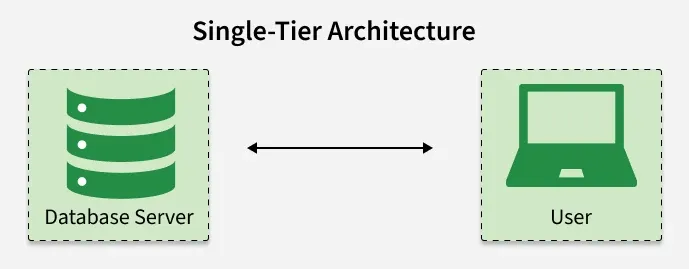
\includegraphics[width=0.78\textwidth,height=0.68\textheight,keepaspectratio]{image-1.png}
\vfill
\vspace{0.25cm}
\small \textit{The user interface, processing logic, and data are located on the same computer or within the same application.}
\end{frame}

%------------------------------------------------
\begin{frame}{Example of 1-Tier Architecture}
\small
\begin{block}{Common example}
\keyword{Microsoft Access} is a common example of 1-tier architecture.
\end{block}

In MS Access:
\begin{itemize}
\tightlist
  \item Users enter data directly.
  \item The application processes calculations or queries.
  \item Data is stored directly on the personal computer.
  \item No separate database server is required.
\end{itemize}

\begin{exampleblock}{Suitable for}
Personal applications, standalone applications, small practice projects, or small-scale systems.
\end{exampleblock}
\end{frame}

%------------------------------------------------
\begin{frame}{1-Tier Architecture: Advantages}
\small
\begin{itemize}
\tightlist
  \item \keyword{Simple}: only one computer is needed for installation, operation, and maintenance.
  \item \keyword{Low cost}: no server, network infrastructure, or complex hardware is required.
  \item \keyword{Easy to deploy}: suitable for small projects, individual practice, or simple internal applications.
  \item \keyword{No network dependency}: users can work directly on their personal computer.
\end{itemize}
\end{frame}

%------------------------------------------------
\begin{frame}{1-Tier Architecture: Disadvantages}
\small
\begin{itemize}
\tightlist
  \item \keyword{Suitable mainly for a single user}: not ideal for teamwork or multi-user environments.
  \item \keyword{Weak security}: the application and data are located on the same machine.
  \item \keyword{No centralized control}: data is stored locally, making centralized management and backup difficult.
  \item \keyword{Difficult data sharing}: data is stored on one computer, so sharing it across devices is inconvenient.
\end{itemize}
\end{frame}

%------------------------------------------------
\begin{frame}{Quiz: 1-Tier Architecture}
\small
\textbf{Question 1.} In 1-tier architecture, which components are usually located on the same machine?
\begin{enumerate}
\tightlist
  \qoption{A}{Only the database}
  \qoption{B}{Only the user interface}
  \qoption{C}{The user interface, processing logic, and data}
  \qoption{D}{Only the application server}
\end{enumerate}

\textbf{Question 2.} Which example best fits 1-tier architecture?
\begin{enumerate}
\tightlist
  \qoption{A}{A large e-commerce system}
  \qoption{B}{An MS Access application running on a personal computer}
  \qoption{C}{An online banking system}
  \qoption{D}{A social networking system}
\end{enumerate}
\end{frame}

%------------------------------------------------
\begin{frame}{Quiz: 1-Tier Architecture (cont.)}
\small
\textbf{Question 3.} What is a major disadvantage of 1-tier architecture?
\begin{enumerate}
\tightlist
  \qoption{A}{It is too complex}
  \qoption{B}{It cannot store data}
  \qoption{C}{It is difficult to support multiple users}
  \qoption{D}{It cannot run on a personal computer}
\end{enumerate}
\end{frame}

%------------------------------------------------
\section{2-Tier Architecture}

\begin{frame}{2-Tier Architecture: Concept}
\small
\keyword{2-tier architecture} is similar to a basic \keyword{client-server} model.

\vspace{0.2cm}
In this model:
\begin{itemize}
\tightlist
  \item \keyword{Client}: runs the user interface and application program.
  \item \keyword{Database Server}: stores and processes data.
\end{itemize}

The client-side application communicates directly with the database on the server side. APIs such as \keyword{ODBC} and \keyword{JDBC} are often used to support the connection.
\end{frame}

%------------------------------------------------
\begin{frame}{2-Tier Architecture Diagram}
\centering
\vfill
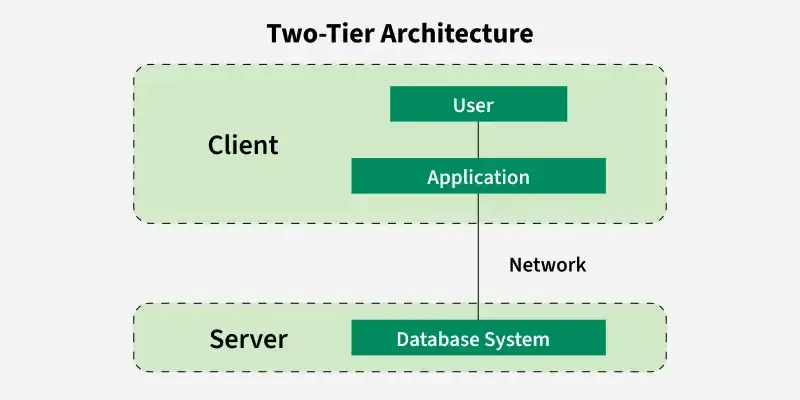
\includegraphics[width=0.78\textwidth,height=0.68\textheight,keepaspectratio]{image-2.png}
\vfill
\vspace{0.5cm}
\small The client connects directly to the database server to send queries and receive results.
\end{frame}

%------------------------------------------------
\begin{frame}{Example: Library Management System}
\small
\begin{columns}[T]
\column{0.48\textwidth}
\begin{block}{Client tier}
A desktop application allows library staff or users to:
\begin{itemize}
\tightlist
  \item Search for books.
  \item Borrow books.
  \item Return books.
  \item Check due dates.
\end{itemize}
\end{block}

\column{0.48\textwidth}
\begin{block}{Database tier}
The database server stores:
\begin{itemize}
\tightlist
  \item Book information.
  \item User information.
  \item Borrowing and returning history.
  \item Transaction logs.
\end{itemize}
\end{block}
\end{columns}
\end{frame}

%------------------------------------------------
\begin{frame}{2-Tier Architecture: Advantages}
\small
\begin{itemize}
\tightlist
  \item \keyword{Fast data access}: the client can send queries directly to the server.
  \item \keyword{Lower cost than 3-tier}: no intermediate application tier is required.
  \item \keyword{Easy to deploy}: the model consists only of client and database server.
  \item \keyword{Simple}: suitable for small or medium systems within an internal network.
\end{itemize}
\end{frame}

%------------------------------------------------
\begin{frame}{2-Tier Architecture: Disadvantages}
\small
\begin{itemize}
\tightlist
  \item \keyword{Limited scalability}: the server may become overloaded as the number of clients increases.
  \item \keyword{Security issues}: clients connect directly to the database.
  \item \keyword{Tight coupling}: when the database changes, the client often needs to be updated.
  \item \keyword{Difficult maintenance}: updates, bug fixes, and feature additions become harder as the number of clients grows.
\end{itemize}
\end{frame}

%------------------------------------------------
\begin{frame}{Quiz: 2-Tier Architecture}
\small
\textbf{Question 1.} What are the two main tiers in 2-tier architecture?
\begin{enumerate}
\tightlist
  \qoption{A}{Client and database server}
  \qoption{B}{Client and web browser}
  \qoption{C}{Database and operating system}
  \qoption{D}{Application and text file}
\end{enumerate}

\textbf{Question 2.} In 2-tier architecture, which technologies are often used by the client to communicate with the database?
\begin{enumerate}
\tightlist
  \qoption{A}{HTML and CSS}
  \qoption{B}{ODBC or JDBC}
  \qoption{C}{Bluetooth}
  \qoption{D}{FTP}
\end{enumerate}
\end{frame}

%------------------------------------------------
\begin{frame}{Quiz: 2-Tier Architecture (cont.)}
\small
\textbf{Question 3.} What is a security disadvantage of 2-tier architecture?
\begin{enumerate}
\tightlist
  \qoption{A}{It cannot store data}
  \qoption{B}{The client connects directly to the database}
  \qoption{C}{It has no user interface}
  \qoption{D}{It cannot process queries}
\end{enumerate}
\end{frame}

%------------------------------------------------
\section{3-Tier Architecture}

\begin{frame}{3-Tier Architecture: Concept}
\small
In \keyword{3-tier architecture}, an intermediate layer is added between the client and the database server.

\vspace{0.2cm}
The three main tiers are:
\begin{enumerate}
\tightlist
  \item \keyword{Presentation Layer}.
  \item \keyword{Application / Business Logic Layer}.
  \item \keyword{Database Layer}.
\end{enumerate}

The client does not communicate directly with the database. Instead, the client sends requests to the application server.
\end{frame}

%------------------------------------------------
\begin{frame}{3-Tier Architecture Diagram}
\centering
\vfill
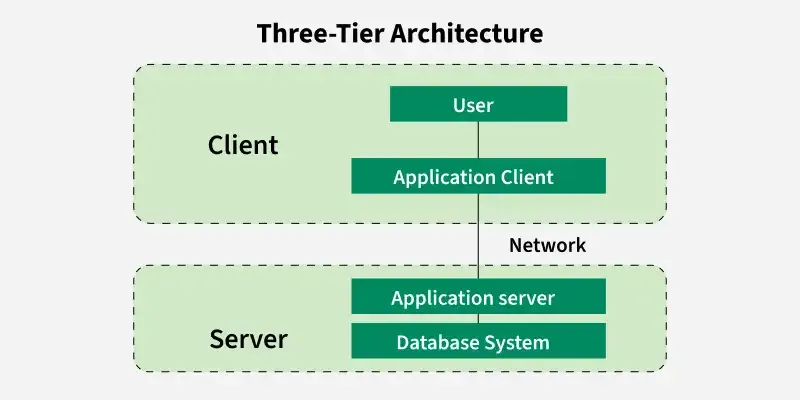
\includegraphics[width=0.78\textwidth,height=0.68\textheight,keepaspectratio]{image-3.png}
\vfill
\vspace{0.5cm}
\small The application tier acts as an intermediary that controls business logic and data access.
\end{frame}

%------------------------------------------------
\begin{frame}{Processing Flow in 3-Tier Architecture}
\small
\begin{enumerate}
\tightlist
  \item The client sends a request to the application server.
  \item The application server processes business logic.
  \item The application server sends a query to the database server when needed.
  \item The database server returns data to the application server.
  \item The application server processes the result and sends a response back to the client.
\end{enumerate}

\begin{block}{Common applications}
3-tier architecture is often used in large web applications, enterprise systems, e-commerce platforms, online banking, and systems with many concurrent users.
\end{block}
\end{frame}

%------------------------------------------------
\begin{frame}{Example: E-Commerce Store}
\small
\begin{columns}[T]
\column{0.33\textwidth}
\begin{block}{User}
\begin{itemize}
\tightlist
  \item Visits the website.
  \item Searches for products.
  \item Adds items to the cart.
\end{itemize}
\end{block}

\column{0.33\textwidth}
\begin{block}{Processing tier}
\begin{itemize}
\tightlist
  \item Checks inventory.
  \item Calculates total price.
  \item Applies discounts.
  \item Authenticates accounts.
\end{itemize}
\end{block}

\column{0.33\textwidth}
\begin{block}{Data tier}
\begin{itemize}
\tightlist
  \item Products.
  \item Customers.
  \item Shopping carts.
  \item Orders.
\end{itemize}
\end{block}
\end{columns}
\end{frame}

%------------------------------------------------
\begin{frame}{3-Tier Architecture: Advantages}
\small
\begin{itemize}
\tightlist
  \item \keyword{Better scalability}: the application tier can be distributed across multiple servers.
  \item \keyword{Improved data integrity}: the middle tier validates data before sending it to the database.
  \item \keyword{Better security}: clients do not access the database directly.
  \item \keyword{Easier maintenance}: business logic is placed in the application tier.
  \item \keyword{Suitable for large applications}: supports many users, many functions, and high security requirements.
\end{itemize}
\end{frame}

%------------------------------------------------
\begin{frame}{3-Tier Architecture: Disadvantages}
\small
\begin{itemize}
\tightlist
  \item \keyword{More complex}: it has an additional middle tier compared with 2-tier architecture.
  \item \keyword{More difficult communication design}: data must pass through multiple tiers.
  \item \keyword{Response time may be slower}: requests must go through the application server.
  \item \keyword{Higher cost}: more hardware, software, and specialized personnel are required.
\end{itemize}
\end{frame}

%------------------------------------------------
\begin{frame}{Quiz: 3-Tier Architecture}
\small
\textbf{Question 1.} What are the three main tiers in 3-tier architecture?
\begin{enumerate}
\tightlist
  \qoption{A}{File, folder, disk}
  \qoption{B}{Client, application server, database server}
  \qoption{C}{RAM, CPU, hard disk}
  \qoption{D}{User, password, table}
\end{enumerate}

\textbf{Question 2.} In 3-tier architecture, does the client connect directly to the database?
\begin{enumerate}
\tightlist
  \qoption{A}{Yes}
  \qoption{B}{No}
  \qoption{C}{Only when the database is small}
  \qoption{D}{Only when using MS Access}
\end{enumerate}
\end{frame}

%------------------------------------------------
\begin{frame}{Quiz: 3-Tier Architecture (cont.)}
\small
\textbf{Question 3.} What is the main security benefit of 3-tier architecture?
\begin{enumerate}
\tightlist
  \qoption{A}{No password is needed}
  \qoption{B}{The client does not access the database directly}
  \qoption{C}{No server is needed}
  \qoption{D}{Data is stored on paper}
\end{enumerate}
\end{frame}

%------------------------------------------------
\section{Comparison and Selection}

\begin{frame}{Quick Comparison of Three Architectures}
\scriptsize
\begin{tabularx}{\textwidth}{p{0.20\textwidth} X X X}
\toprule
\textbf{Criterion} & \textbf{1-Tier} & \textbf{2-Tier} & \textbf{3-Tier} \\
\midrule
Number of tiers & 1 & 2 & 3 \\
Components & Application and data on the same machine & Client and database server & Client, application server, database server \\
Data access & Directly on the local machine & Client directly to database server & Through application server \\
Example & Personal MS Access app & Small library management system & E-commerce website \\
Scalability & Low & Medium & High \\
Security & Low & Medium & Better \\
\bottomrule
\end{tabularx}
\end{frame}

%------------------------------------------------
\begin{frame}{When Should Each Architecture Be Used?}
\small
\begin{columns}[T]
\column{0.32\textwidth}
\begin{block}{1-Tier}
\begin{itemize}
\tightlist
  \item Personal applications.
  \item Small data.
  \item Single user.
  \item Low cost.
\end{itemize}
\end{block}

\column{0.32\textwidth}
\begin{block}{2-Tier}
\begin{itemize}
\tightlist
  \item Small or medium organizations.
  \item Internal network.
  \item Desktop applications.
  \item Client connects to DB.
\end{itemize}
\end{block}

\column{0.32\textwidth}
\begin{block}{3-Tier}
\begin{itemize}
\tightlist
  \item Large web applications.
  \item Many users.
  \item High security.
  \item Easy scalability.
\end{itemize}
\end{block}
\end{columns}
\end{frame}

%------------------------------------------------
\begin{frame}{Review Questions: Multiple Choice 1-3}
\small
\textbf{Question 1.} What does DBMS architecture describe?
\begin{enumerate}\tightlist
  \qoption{A}{How to design graphical interfaces}
  \qoption{B}{How users and applications interact with the database}
  \qoption{C}{How to assemble computer hardware}
  \qoption{D}{How to format documents}
\end{enumerate}

\textbf{Question 2.} Which architecture is most suitable for a personal application that does not need a network?
\begin{enumerate}\tightlist
  \qoption{A}{1-tier} \qoption{B}{2-tier} \qoption{C}{3-tier} \qoption{D}{Multi-tier}
\end{enumerate}

\textbf{Question 3.} In 2-tier architecture, what does the client tier usually contain?
\begin{enumerate}\tightlist
  \qoption{A}{User interface and application program}
  \qoption{B}{Only raw data}
  \qoption{C}{Only hard disk}
  \qoption{D}{Only operating system}
\end{enumerate}
\end{frame}

%------------------------------------------------
\begin{frame}{Review Questions: Multiple Choice 4-6}
\small
\textbf{Question 4.} In 3-tier architecture, which tier usually processes business logic?
\begin{enumerate}\tightlist
  \qoption{A}{Presentation tier}
  \qoption{B}{Application tier}
  \qoption{C}{Database tier}
  \qoption{D}{Physical storage tier}
\end{enumerate}

\textbf{Question 5.} What is the main disadvantage of 1-tier architecture?
\begin{enumerate}\tightlist
  \qoption{A}{It cannot store data}
  \qoption{B}{It is difficult to support multiple users and has weak security}
  \qoption{C}{It always requires many servers}
  \qoption{D}{It cannot be used for small applications}
\end{enumerate}

\textbf{Question 6.} Why does 3-tier architecture usually provide better security?
\begin{enumerate}\tightlist
  \qoption{A}{Because it does not need a database}
  \qoption{B}{Because the client does not access the database directly}
  \qoption{C}{Because data is not stored}
  \qoption{D}{Because there is no application tier}
\end{enumerate}
\end{frame}

%------------------------------------------------
\begin{frame}{Review Questions: Multiple Choice 7-8}
\small
\textbf{Question 7.} Which example best fits 3-tier architecture?
\begin{enumerate}\tightlist
  \qoption{A}{An Excel file stored on a personal computer}
  \qoption{B}{MS Access used by one person}
  \qoption{C}{An e-commerce website}
  \qoption{D}{A text file stored on a USB drive}
\end{enumerate}

\textbf{Question 8.} In 2-tier architecture, what problem may occur when the number of users increases significantly?
\begin{enumerate}\tightlist
  \qoption{A}{The server may be overloaded by many direct connections}
  \qoption{B}{The client loses its interface}
  \qoption{C}{The database disappears automatically}
  \qoption{D}{Tables cannot be created}
\end{enumerate}
\end{frame}

%------------------------------------------------
\begin{frame}{Review Questions: Multiple Choice 9-10}
\small
\textbf{Question 9.} In which architecture are ODBC and JDBC commonly used?
\begin{enumerate}\tightlist
  \qoption{A}{1-tier}
  \qoption{B}{2-tier}
  \qoption{C}{3-tier}
  \qoption{D}{Unrelated to DBMS}
\end{enumerate}

\textbf{Question 10.} Which architecture is usually most suitable for large enterprise systems?
\begin{enumerate}\tightlist
  \qoption{A}{1-tier}
  \qoption{B}{2-tier}
  \qoption{C}{3-tier}
  \qoption{D}{File-based system}
\end{enumerate}
\end{frame}

%------------------------------------------------
\begin{frame}{Review Questions: Short Answers}
\small
\begin{enumerate}\tightlist
  \item Why is 1-tier architecture not suitable for systems with many users?
  \item Distinguish between 2-tier and 3-tier architecture in terms of how the client accesses the database.
  \item Why is 3-tier architecture commonly used for large web applications?
  \item Give one real-world example for each type of DBMS architecture.
\end{enumerate}
\end{frame}

%------------------------------------------------
\begin{frame}{Practice Exercise 1}
\small
\begin{block}{Scenario}
A small store wants to manage its product list and sales revenue on a personal computer. The store has only one system user.
\end{block}

\begin{exampleblock}{Task}
Suggest a suitable DBMS architecture and explain your reasoning.
\end{exampleblock}
\end{frame}

%------------------------------------------------
\begin{frame}{Practice Exercise 2}
\small
\begin{block}{Scenario}
A school library wants to build a desktop application that allows multiple staff members to search for books and update borrowing and returning information. The data is stored on a server in the internal network.
\end{block}

\begin{exampleblock}{Task}
Suggest a suitable DBMS architecture and explain your reasoning.
\end{exampleblock}
\end{frame}

%------------------------------------------------
\begin{frame}{Practice Exercise 3}
\small
\begin{block}{Scenario}
A company wants to build an e-commerce website serving thousands of concurrent users. The system needs security, order processing, inventory checking, and purchase history storage.
\end{block}

\begin{exampleblock}{Task}
Suggest a suitable DBMS architecture and explain your reasoning.
\end{exampleblock}
\end{frame}

%------------------------------------------------
\begin{frame}{Lesson Summary}
\small
\begin{itemize}
\tightlist
  \item DBMS architecture describes how users, applications, and databases interact.
  \item 1-tier architecture is simple and low-cost but has weak scalability and security.
  \item 2-tier architecture includes a client and database server and is suitable for small or medium systems.
  \item 3-tier architecture adds an application server, improving security, scalability, and maintainability.
  \item The choice of architecture depends on system size, number of users, security requirements, cost, and scalability.
\end{itemize}
\end{frame}

%------------------------------------------------
\begin{frame}{Key Terms}
\small
\begin{columns}[T]
\column{0.5\textwidth}
\begin{itemize}\tightlist
  \item DBMS Architecture
  \item 1-Tier Architecture
  \item 2-Tier Architecture
  \item 3-Tier Architecture
  \item Client
  \item Server
  \item Database Server
  \item Application Server
\end{itemize}

\column{0.5\textwidth}
\begin{itemize}\tightlist
  \item Presentation Layer
  \item Business Logic Layer
  \item Database Layer
  \item ODBC
  \item JDBC
  \item Scalability
  \item Security
  \item Data Integrity
\end{itemize}
\end{columns}
\end{frame}

\end{document}
